% !TeX root = ../main.tex
% Add the above to each chapter to make compiling the PDF easier in some editors.

\chapter{Related Works}\label{chapter:related_works}


\section{Traditional Approaches for Prognostic and Health Management}

Traditionally, model-based and data-driven models were used as PHM systems. Model-based methods predict the health condition based on physical models, which describe the underlying mechanisms of degradation. Uncertainties in the machine processes as well as noise make the application of physical models difficult. Often, the identification of all model parameters is difficult and requires a lot of experiments. Data-driven methods learn a mapping relationship between the health condition state and monitoring data. Such methods do not use physical information about the degradation process. The performance of data-driven approaches highly depends on the quality and amount of the training data. Besides that, data-driven models might lack from generality. The models are just optimized to perform well on the working conditions, which are present in the train data. Both, model-based and data-driven approaches suffer from different limitations \cite{DENG2020}. In the following, data-driven and model-based approaches in the context of PHM for BSDs are presented. 

\subsection{Model-Based Approach: Defect Frequency Estimation Based on a Model Simplification of Ball Screw Drives as Rolling Bearings}
Lee et al. \cite{Lee2015} proposed a diagnosis system, which estimates the flaking degradation of BSD shafts. By filtering the machine signals for previously calculated characteristic defect frequencies, the severity and location of the degradation can be predicted. Lee et al. developed a testbed containing one BSD and linear motion guides. An accelerometer was mounted on the BSD nut. Holes with a diameter of 3 mm were punched in the BSD shaft to simulate the degradation. The continous process of fatigue was modeled by increasing the number of holes in the BSD shaft. Each time the steel balls of the BSD pass a whole in the surface of the BSD shaft, the machine signal shows a corresponding defect pattern. The motor was actuated with a constant velocity while the data was recorded. Harris and McCool \cite{Harris1996} proposed a method to estimate the characteristic defect frequencies of rolling bearings. Lee et al. \cite{Lee2015} extended that method to make it applicable for BSDs. BSD screw shafts are considered as inner and the BSD nuts as outer rings of rolling bearings. From the BSD construction details and relative speeds, defect frequencies can be calculated. The ball pass frequencies of the shaft (BPFS) and nut (BPFN), as well as the ball spin frequency (BSF) are considered as defect frequency: 
\begin{equation}
    BPFS = \frac{1}{120}zn(1+\frac{D_{w}}{d_{m}}cos\alpha),
    \label{eq:defect_frequency}
\end{equation}
\begin{equation}
    BPFN = \frac{1}{120}zn(1-\frac{D_{w}}{d_{m}}cos\alpha),
\end{equation}
\begin{equation}
    BSF = \frac{1}{120}n\frac{d_{m}}{D_{w}} (1-\frac{D_{w}}{d_{m}}cos\alpha)(1+\frac{D_{w}}{d_{m}}cos\alpha) ,
\end{equation}
where $\alpha$ is the contact angle between the ball, nuts and screw shaft, $d_{m}$ is the pitch diameter of the balls, $D_{w}$ is the diameter of a single ball, the rotational speeds of external and internal races are defined by $n_{e}$ and $n_{i}$ and $z$ is the number of steel balls. A more detailed visualization of the bearing parameters is shown in fig. \ref{fig:defect_frequency_calc}. 

\begin{figure}[H]
  \centering
  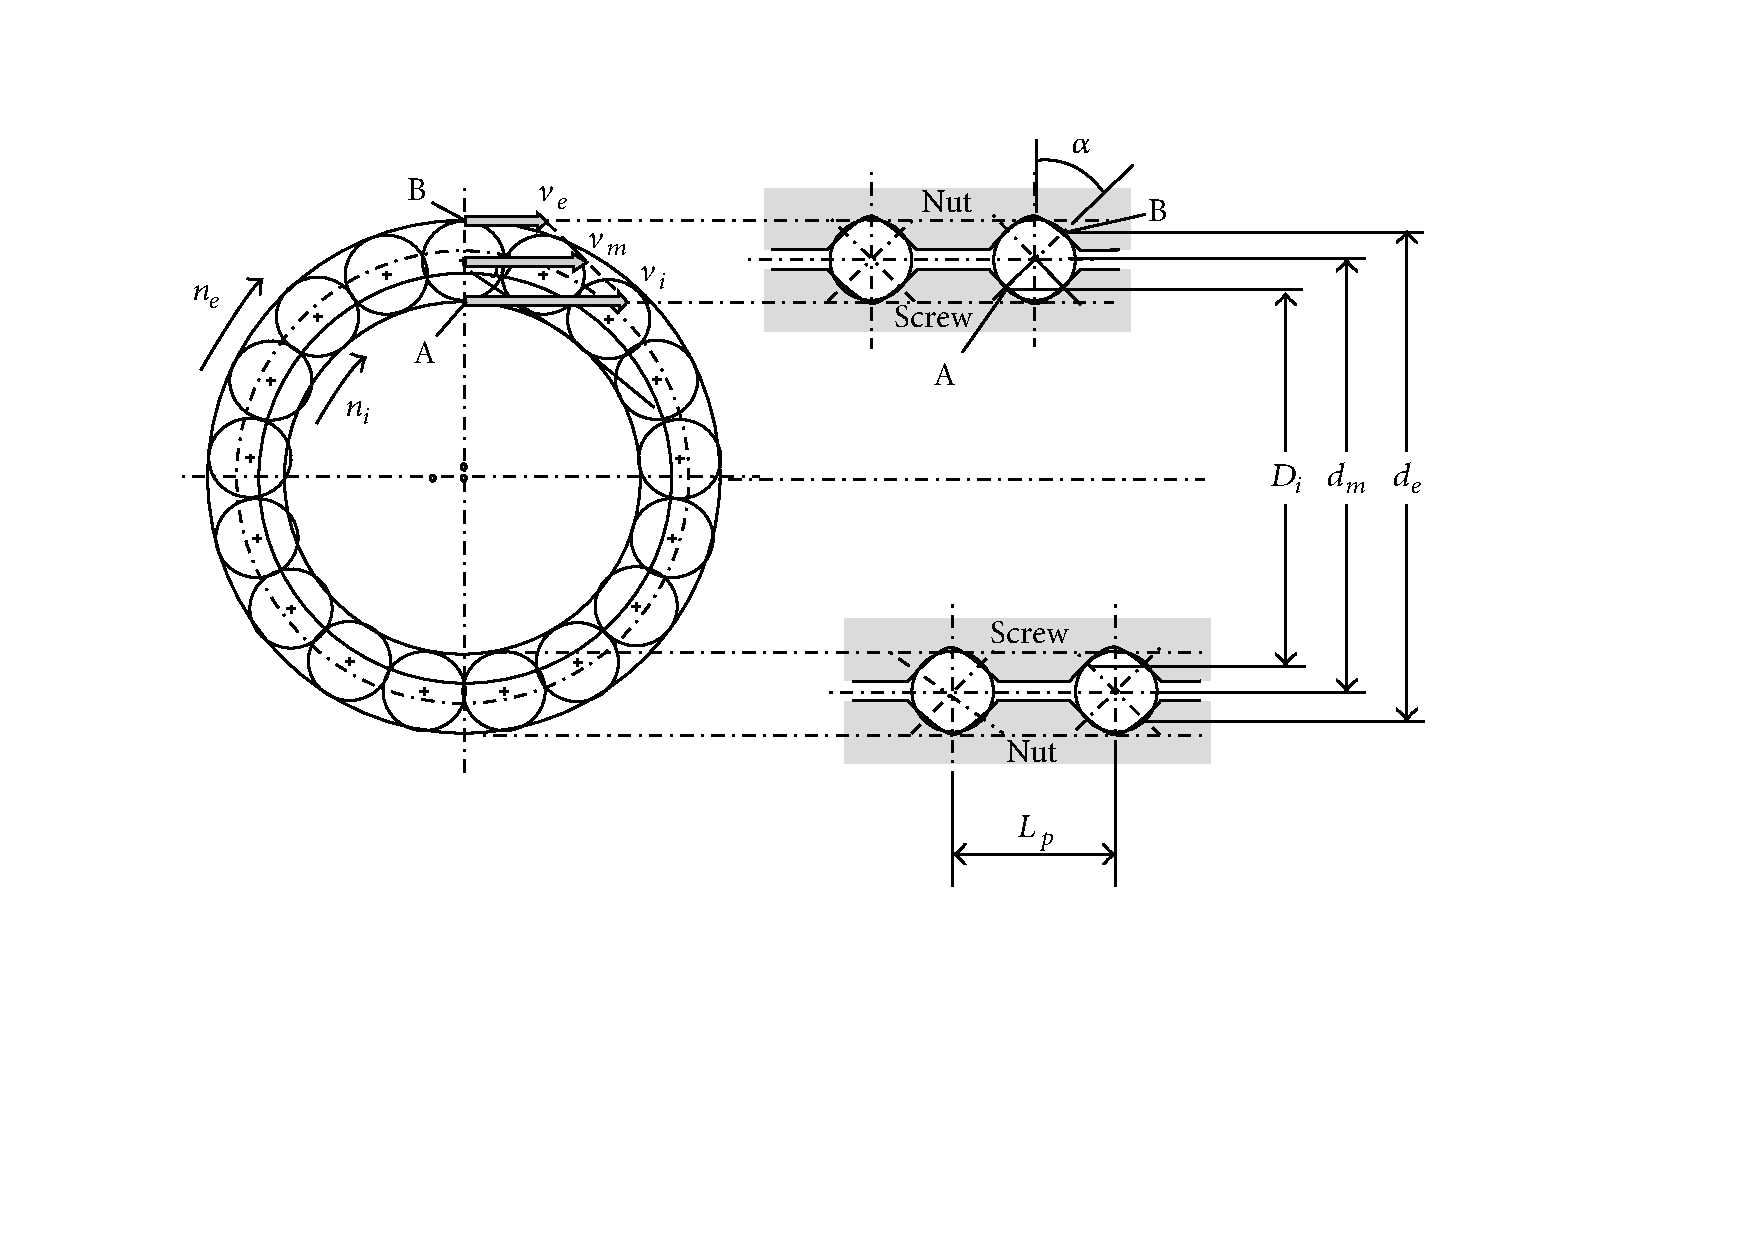
\includegraphics[width=.6\textwidth]{models_state_of_the_art/defect_frequency_calc.pdf}
  \caption{Simplification of BSDs as bearings for frequency calculation \cite{Lee2015}}
  \label{fig:defect_frequency_calc}
\end{figure}

The above derived frequencies are valid for rolling bearings. To apply those to BSDs one has to replace $z$ and $d_{m}$ by the effective number of steel balls $z^{'}$ and effective pitch parameter $d_{m}^{'}$, which are defined as following:

\begin{equation}
    d_{m}^{'} = (L_{p}^{2}+(\pi D_{b})^{2})^{\frac{1}{2}},
\end{equation}
\begin{equation}
    z^{'} = \frac{d_{m}^{'}}{D_{w}}.
\end{equation}
The translation between the regular and effective parameters is visualized in fig. \ref{fig:defect_frequency_transfer}. 

\begin{figure}[H]
  \centering
  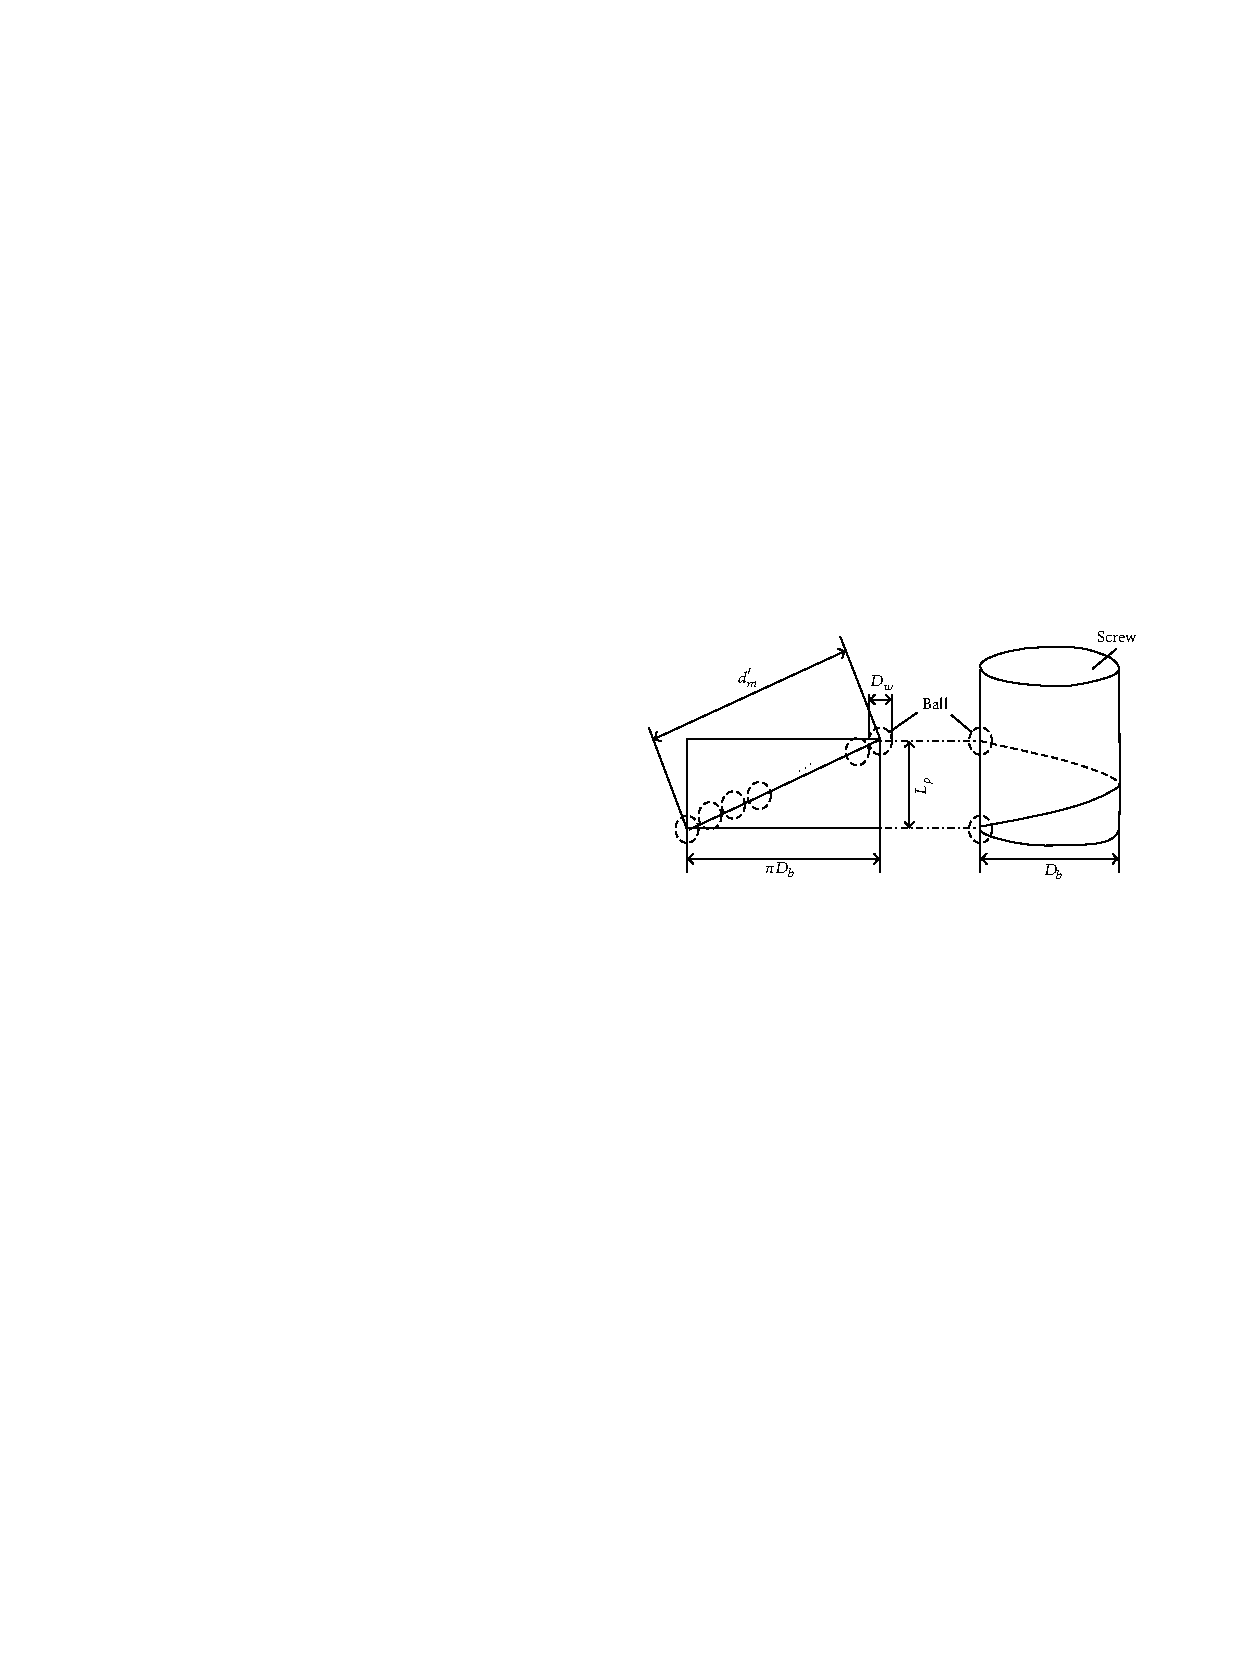
\includegraphics[width=.7\textwidth]{models_state_of_the_art/defect_frequency_transfer.pdf}
  \caption{Transfering pitch parameter and number of steel balls from bearings to BSDs \cite{Lee2015}}
  \label{fig:defect_frequency_transfer}
\end{figure}

The BPFS frequency was identified as the most expressive and reliable one for supervising the health condition of BSDs. To calculate the BPFS for ball screw drives the equation \ref{eq:defect_frequency} must be combined with the effective pitch parameter $d_{m}^{'}$ and effective number of steel balls $z^{'}$. During testing, the wavelet transform (Daubechies Wavelet (db14) function) is used to transform the machine signals in the two-dimensional time-frequency domain. By supervising the magnitude of the calculated defect frequency in the time-frequency domain of the machine signal, the degradation status of the BSD can be monitored. An alarm is triggered when the degradation is not acceptable anymore. The time-related information are an indicator for detect location. The frequency-related information provide information about the degradation status of the BSD. The proposed approach during testing is again visualized in fig. \ref{fig:defect_frequency_model}. 


\begin{figure}[H]
  \centering
  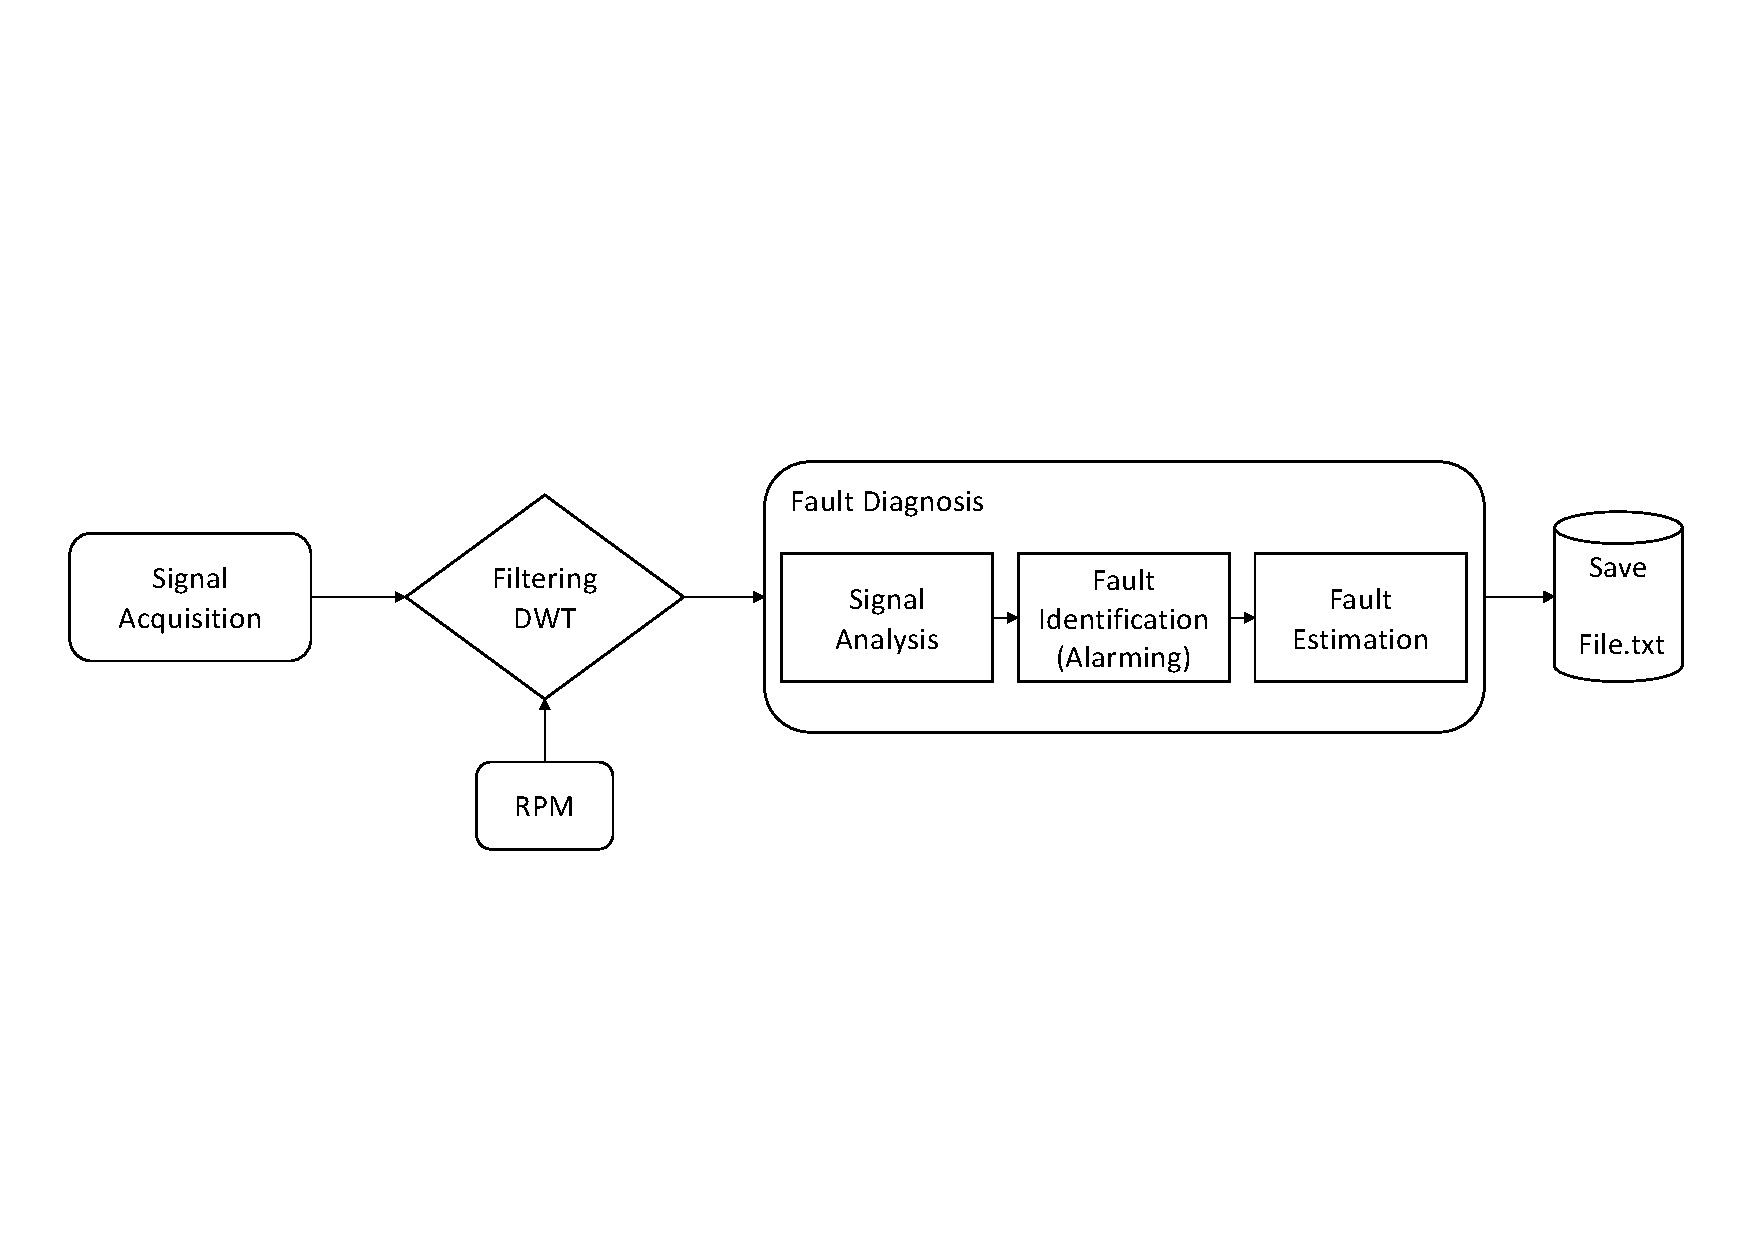
\includegraphics[width=.95\textwidth]{models_state_of_the_art/defect_frequency_model.pdf}
  \caption{Failure diagnosis system by monitoring defect frequencies based on \cite{Lee2015}}
  \label{fig:defect_frequency_model}
\end{figure}

\subsubsection{Conclusion}
Lee et al. \cite{Lee2015} assume that defects and degradation are mainly subjected to rolling friction. Often times such simplifying assumptions are made when developing model-based PHM systems. In reality the balls in BSDs are rotating, revolving, and sliding \cite{Lee2015}. These highly complex processes make the accurate modeling of the degradation, which is essential to achieve a good PHM performance, more challenging. In data-driven PHM systems the correlation between the machine data and degradation patterns can be learned flexibly. By picking appropriate signals and classes the PHM system can be adapted to predict different degradation patterns and levels. Lee et al. \cite{Lee2015} have to stick to the defect frequency definitions by Harris et al. \cite{Harris1996}, which just consider the flaking related degradation of BSDs. Adapting the diagnosis system to monitor other degradation types is hardly possible. When comparing the frequencies extracted from machine signals with the calculated defect frequencies, Lee et al. observed other distinct frequencies coming from major electrical noise. The proposed method was just tested on a simplified BSD testbed. When applying the approach on real-world machines, vibrations from other components might contaminate the recorded signal. Distinguishing the characteristic frequencies from different components then becomes even more challenging. The accelerometer, recording the BSD vibration signals, was mounted on the BSD nut. The BSD nut is a highly fault-critical sensor location, but it is also very impractical for the real-world use \cite{Pandhare2021}. It is questionable, how this method would work with vibration signals recorded from less fault-critical sensor locations. Finding all parameters to calculate the defect frequencies might require a lot of measuring and testing effort. Often these parameters are assumed to be constant throughout the lifetime of BSDs. The rolling diameter for example will be reduced throughout the lifetime of a rolling bearing. Anyhow, this parameter is used as a constant parameter in the calculation of the defect frequencies of BSDs. When transferring the calculated defect frequencies from the rolling bearing to the BSD only structural differences are considered. The linear movement of BSDs is completely ignored, which represents a fundamental functional difference between rolling bearings and BSDs. The degradation process was simulated by punching holes with a diameter of 3 mm on the grooves of the BSD shaft. Solely the number of holes simulates the degradation problem. Variations in the dimension of these holes were not considered. In total it is disputable whether the degradation is simulated appropriately.  

\subsection{Model-Based Approach: Discrete Dynamic Modeling}
Nguyen et al. \cite{NGUYEN2019} applied a simplified dynamic model (see fig. \ref{fig:Nguyen_discrete_dynamic_model}) to investigate the relation between the preload variations and dynamic characteristics in BSDs.

\begin{figure}[H]
  \centering
  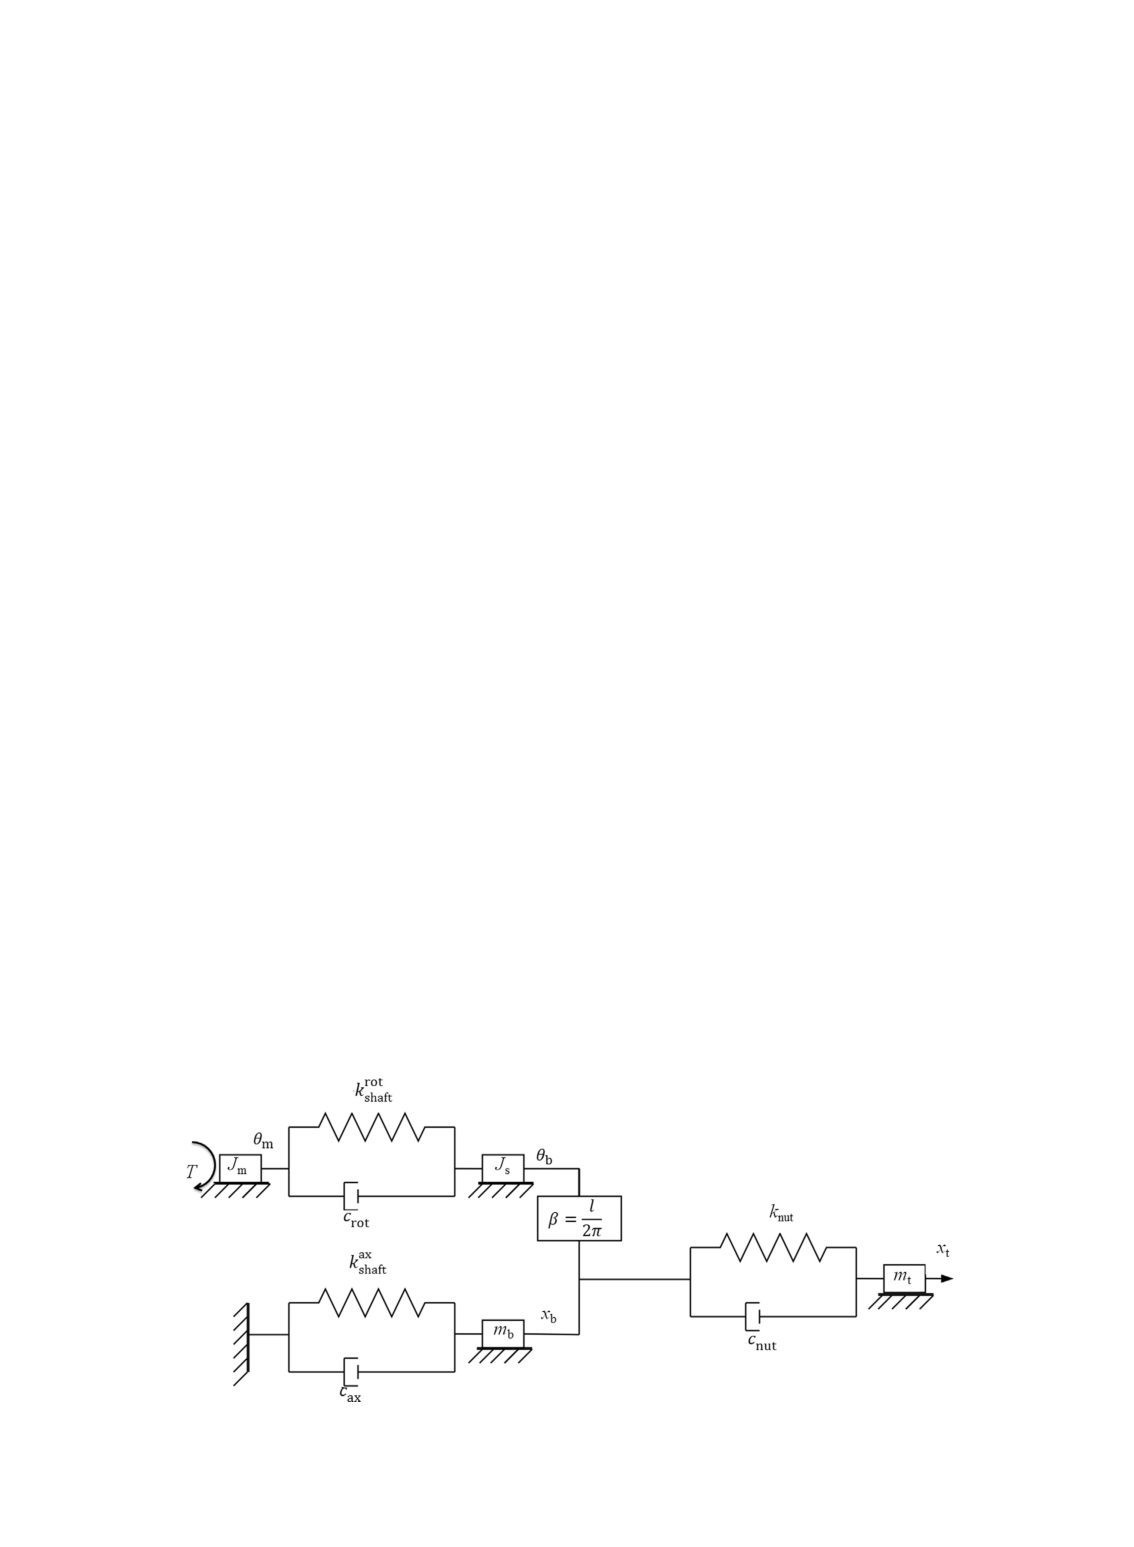
\includegraphics[width=1\textwidth]{models_state_of_the_art/Nguyen_discrete_dynamic_model.pdf}
  \caption{discrete dynamic model \cite{NGUYEN2019}}
  \label{fig:Nguyen_discrete_dynamic_model}
\end{figure}

According to the discrete dynamic model the BSD preload variations correlate with the screw nut stiffness:

\begin{equation}
    k_{nut}=0.8K(\frac{P}{0.1C_{a}})^{\frac{1}{3}},
\end{equation}

where $P$ is the BSD preload, $C_{a}$ is the BSD screw dynamic load, $K$ is the BSD nut stiffness according to the manufacturer and $k_{nut}$ is the actual BSD nut stiffness. The formula is valid if the BSD preload is less than 10\% of the BSD dynamic load. The axial and rotational stiffness of the BSD shaft is defined by the configuration parameters and the working table displacement:
\begin{equation}
    k_{shaft}^{ax}=\frac{EA}{x_{t}}=\frac{\pi}{4x_{t}}d_{minor}^{2}E,
\end{equation}
\begin{equation}
    k_{shaft}^{rot}=\frac{\pi}{32L}d_{minor}^{4}G,
\end{equation}
 where $A$ is the cross sectional area of the BSD shaft, $E$ the Young’s modulus, $d_{minor}$ the screw diameter, $G$ the shear modulus, $L$ the screw shaft length and $x_{t}$ the working table displacement. The total axial stiffness of the BSD is composed of the stiffness of the screw shaft, supporting bearing, screw nut, and bracket:
 \begin{equation}
    \frac{1}{k_{ax}}=\frac{1}{k_{shaft}^{ax}}+\frac{1}{k_{bearing}^{ax}}+\frac{1}{k_{nut}^{ax}}+\frac{1}{k_{bracket}^{ax}}+\frac{1}{\frac{k_{shaft}^{rot}}{\beta^{2}}}.
\end{equation}
From there, the axial natural frequency is calculated based of the axial stiffness and mass of the ball screw system:
\begin{equation}
    f\approx\frac{1}{2\pi}\sqrt{\frac{k_{ax}}{m_{table}+m_{screw}+m_{nut}+m_{bracket}}}=\frac{1}{2\pi}\sqrt{\frac{k_{ax}}{\sum M}}.
\end{equation}

According to the discrete dynamic model, the BSD preload can be estimated from the axial natural frequency, the mass and displacement of the ball screw system and some other configuration parameters:
\begin{equation}
    P=\frac{0.1C_{a}}{\{0.8K[ -\frac{4x_{t}}{\pi d_{minor}^{2}E} -\frac{32\pi^{2}L}{\pi d_{minor}^{4}G}-\frac{1}{k_{bearing}}-\frac{1}{k_{bracket}}+\frac{1}{(2\pi f)^{2}\sum M} ]\}^{3}}
\label{eq:preload_estimation_based_natural_frequency}
\end{equation}
The axial natural frequency increases with the preload and decreases with the mass of the working table. Based on the formulas derived from the simplified discrete dynamic model, a monitoring system was established, which extracts the axial natural frequency from the machine data and calculates the corresponding BSD preload according to equation \ref{eq:preload_estimation_based_natural_frequency}. The monitoring system is separated in different processing phases. Firstly, the vibration and motor current signals are measured with an uni-axial acceleration sensor mounted on the screw nut and three Hall-effect based current sensors. Especially when the motor speed changes rapidly, the modal modes of the BSD system, including the axial natural frequency, are activated strongly. In these phases the deformation of the BSD system is strong enough to make the modal modes of the BSD observable and distinguishable from those of the other components. A trigger is implemented to detect the phases of rapid motor speed change. During those phases, the vibration and motor current signal are recorded and windowed afterwards. The FFT transform is applied to extract an auto-spectrum and cross-spectrum for each window. By averaging the FFT transforms from several occurences at the same positions along the BSD shaft, more stable results are achieved, which are less prone to noise. From those spectra, the frequency response function (FRF) is composed. The calculation of the averaged FRF is visualized in fig. \ref{fig:Nguyen_frf}. The axial natural frequency is the frequency in the FRF with maximum magnitude, which can be found by a peak detection algorithm. The proposed method was evaluated on a simplified testbed under different BSD preload level scenarios \cite{NGUYEN2019}.

\begin{figure}[H]
  \centering
  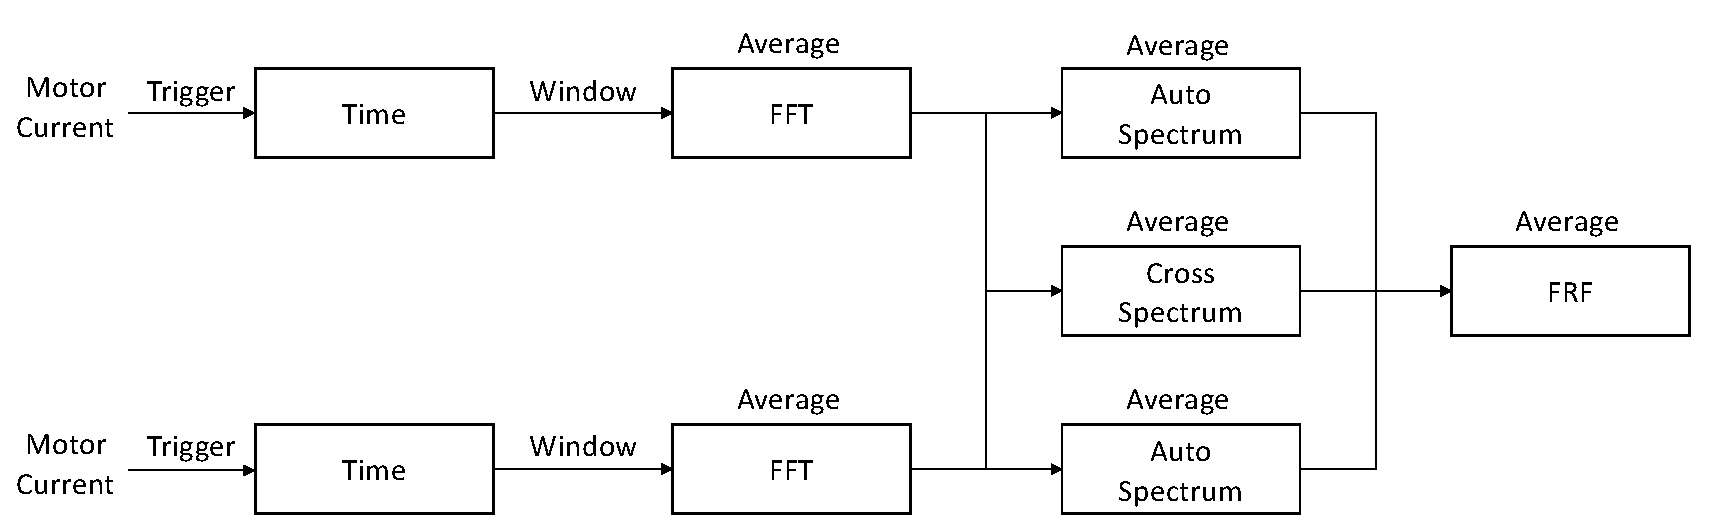
\includegraphics[width=.8\textwidth]{models_state_of_the_art/Nguyen_FRF.pdf}
  \caption{Average FRF calculation \cite{NGUYEN2019}}
  \label{fig:Nguyen_frf}
\end{figure}

\subsubsection{Conclusion}
Nguyen et al. \cite{NGUYEN2019} developed a complex inspection procedure to predict the preload of BSDs. The discrete dynamic model presented in fig. \ref{fig:Nguyen_discrete_dynamic_model} is the base of the preload prediction. The BSD system is simplified by springs and dampers. The preload prediction highly depends on the accuracy of the model and its closeness to the real-world BSD. The modes of the BSD system are activated just in extreme cases, where the motor changes its velocity rapidly. Just in these cases the BSD modes are dominant enough to become visible and distinguishable from those of other components. The proposed BSD diagnosis was evaluated in a very supervised and isolated testbed. When inspecting BSDs installed in big industrial machines, the extraction of the axial natural frequency might become more challenging. The vibration from several other components might disturb the estimation of the BSD modes even more. The goal of such monitoring systems is the continuous estimation of the BSD preload over long time horizons. Operational conditions of the industrial machines might not stay constant throughout those time horizons. The established relationship between the axial natural frequency, the displacement of the working table and the BSD preload might then not be reliable anymore. Even in the proposed isolated BSD testbed, the trigger sometimes failed to detect expressive operational phases for estimating the axial natural frequency. Implementing such a trigger for the BSDs in big industrial machines might be even more difficult. Nguyen et al. \cite{NGUYEN2019} emphasize that at least 10 trigger events from each position along the BSD shaft are required to properly average the FRF in practical applications. Collecting this big amount of trigger events involves a lot of effort and time. Equally to the work of Lee et al. \cite{Lee2015}, the BSD nut is used to record the vibration signal. It was not evaluated whether the axial natural frequency could also be extracted from vibrations signals, which are recorded by sensor mounted in less fault-critical sensor location. In the experiments the BSD preload is changed by a built-in preload adjustment mechanism. The physical degradation of the shaft and the ball surfaces is neglected in the experiments.

\subsection{Data-Driven Approach: Principal Component Analysis based Sensor Fusion of Multiple Statistical Features}

Denkena et al. \cite{Denkena2021} present a method to monitor the preload of BSDs. Firstly, several hand-crafted statistical features are extracted from the machine signals. Afterwards, each feature is rated based on their robustness and statistical significance. The most promising signals are selected and fused based on the principal component analysis (PCA). In the end, decision trees solve the classification task. A testbed consisting of a single BSD and linear guideways was used to evaluate the proposed approach. The BSD preload loss was simulated by installing ball sets with different oversize. Internal control signals were provided by the internal controller and three uniaxial acceleration sensors measure vibrations in the system. The machine data was recorded during constant feed rate over the whole length of the test bench. The proposed PHM method can be separated in four steps:

\begin{itemize}
    \item [\textbf{Data acquisition:}] The method simultaneously processes vibration signals from three uniaxial acceleration sensors as well as internal control signals. The signals are concatenated, synchronized and separated in phases of zero acceleration (constant movement of BSD nut on the BSD shaft) and non-zero acceleration (direction change movement of the BSD nut at each end of the BSD shaft). In the experiments, the ball screw was moved over the length of the test bench with various feed rates (6000 mm/min, 11000 mm/min, 17000 mm/min, 20000 mm/min) \cite{Denkena2021}.
    \item [\textbf{Feature extraction:}] Information about the preload classes are extracted through statistical features (e.g. kurtosis, median, impulse factor, ...). The features are extracted from each signal and segment. At this point the features are unrated. Each feature is evaluated by its robustness and statistical significance. The robustness is measured by the feature's dispersion around the median. After normalizing the feature with the z-score, the significance is estimated by the f-statistics.
    
    \begin{equation}
        \textbf{Z-score:}\qquad \tilde{x}_{i,j} = \frac{x_{i,j} - \bar x_{i}}{\sigma_{i}},
    \end{equation}
    
    \begin{equation}
        \textbf{F-statistic:}\qquad f = \frac{\sum_{j=1}^{J} i \cdot (\bar x_{j} -\bar x)^{2}/(J-1)}{\sum_{j=1}^{J} \sum_{i=1}^{I} i \cdot (\bar x_{j,i} -\bar x_{j})^{2}/(J \cdot (I-1))},
    \end{equation}
    where ${x}_{i,j}$ denotes the feature value j of a sample of class i, $\bar{x}_{i}$ is the feature mean value of class i, ${s}_{i}$ is the feature standard deviation of class i and $\bar{x}$ is the overall feature and class mean value, I and J is the number of all classes and features.  Features are seen as eligible for the diagnosing system, if the dispersion around the median is smaller than $\pm$ 10 and the f-statistics is higher than a critical value of 10 \cite{Denkena2021}. 
    
    \item [\textbf{Principal Component Ananylsis:}] 
    PCA is a method to reduce the dimension of data while retaining most of the information. Principle components are the directions in the feature space, along which the variation of the data is maximal. By using just a few principal components, each sample can be represented by a small number of variables \cite{Ringner2008}. By applying PCA, the selected features are merged with the goal of maintaining the robustness and increasing the f-statistics \cite{Denkena2021}.
    
    \item [\textbf{Classification:}] Decision trees are used to predict a preload class based on the extracted features. Due to its low classification effort and good traceability, decision trees seem suitable for the classification task. For each signal and segment, a separate decision tree is used \cite{Denkena2021}. 
\end{itemize}

\subsubsection{Conclusion}
In order to find features which work well for predicting the degradation state of BSDs, Denkena et al. \cite{Denkena2021} extracted 1500 features from the signal segments. For feed rates higher than 11000 mm/min, the acceleration signals were not suitable for an accurate prediction of the preload classes. Some univariate features, like MAX, RMS and CRE, were only able to separate some of the defined preload classes. For some extracted statistical features the robustness and statistical significance depended on the signals. This shows, that the suitability of the features generally depends strongly on the working conditions, classes and signals. Therefore, the robustness and applicability of the proposed approach for real-world tasks on industrial machines is questionable. The features did not show a proportional behaviour to the physical degradation. When the features MAX and RMS were applied on the acceleration signals, they increased from C3 through C2 to C1, but decreased towards C0. Often deep learning is criticized for its black box principle and the lack of understanding for the extracted features. Even though one generally understands the hand-crafted features, the meaningfulness of the extracted information depends a lot on the task and signal. The correlation between those features and the physical degradation is often highly unknown, which makes such features an equal black box as features extracted by deep learning models. Dekena et al. \cite{Denkena2021} mentioned, that slower feed rates improved the classification performance of some features. Anyhow, one has to remember that those slow feed rates do also increases the inspection time. Generally, one can say that finding a set of features which reliably predicts all BSD preload classes demands quite some effort. These features just work reliable for specific signals, working conditions and preload classes. If any of those specifications change, the whole feature analysis has to be repeated. The physical degradation of the shaft and ball surface is neglected in the experiments.

\subsection{Data-Driven Approach: Multi-Level Feature Selection Module for Health Diagnosis, Assessment and RUL Prediction}
Li et al. \cite{LiPin2018} developed a prognosis system for BSDs, which performs fault diagnosis, early diagnosis, health assessment and remaining useful life (RUL) prediction simultaneously. Since this thesis focuses on the fault diagnosis of BSDs, this chapter is restricted to the processing units related to diagnosis. A testbed was build containing a BSD and horizontal guideways fixed to a concrete base. Instead of manually inserting faults to simulate degradation, it was caused by field use. Fig.  \ref{fig:level_feature_selection_model} shows the different processing steps and the parallel prediction units for the fault diagnosis, health assessment and remaining useful life (RUL) prediction. Vibration data is measured by three accelerometers and speed and torque signals are retrieved from the controller \cite{LiPin2018}. 

\begin{figure}[H]
  \centering
  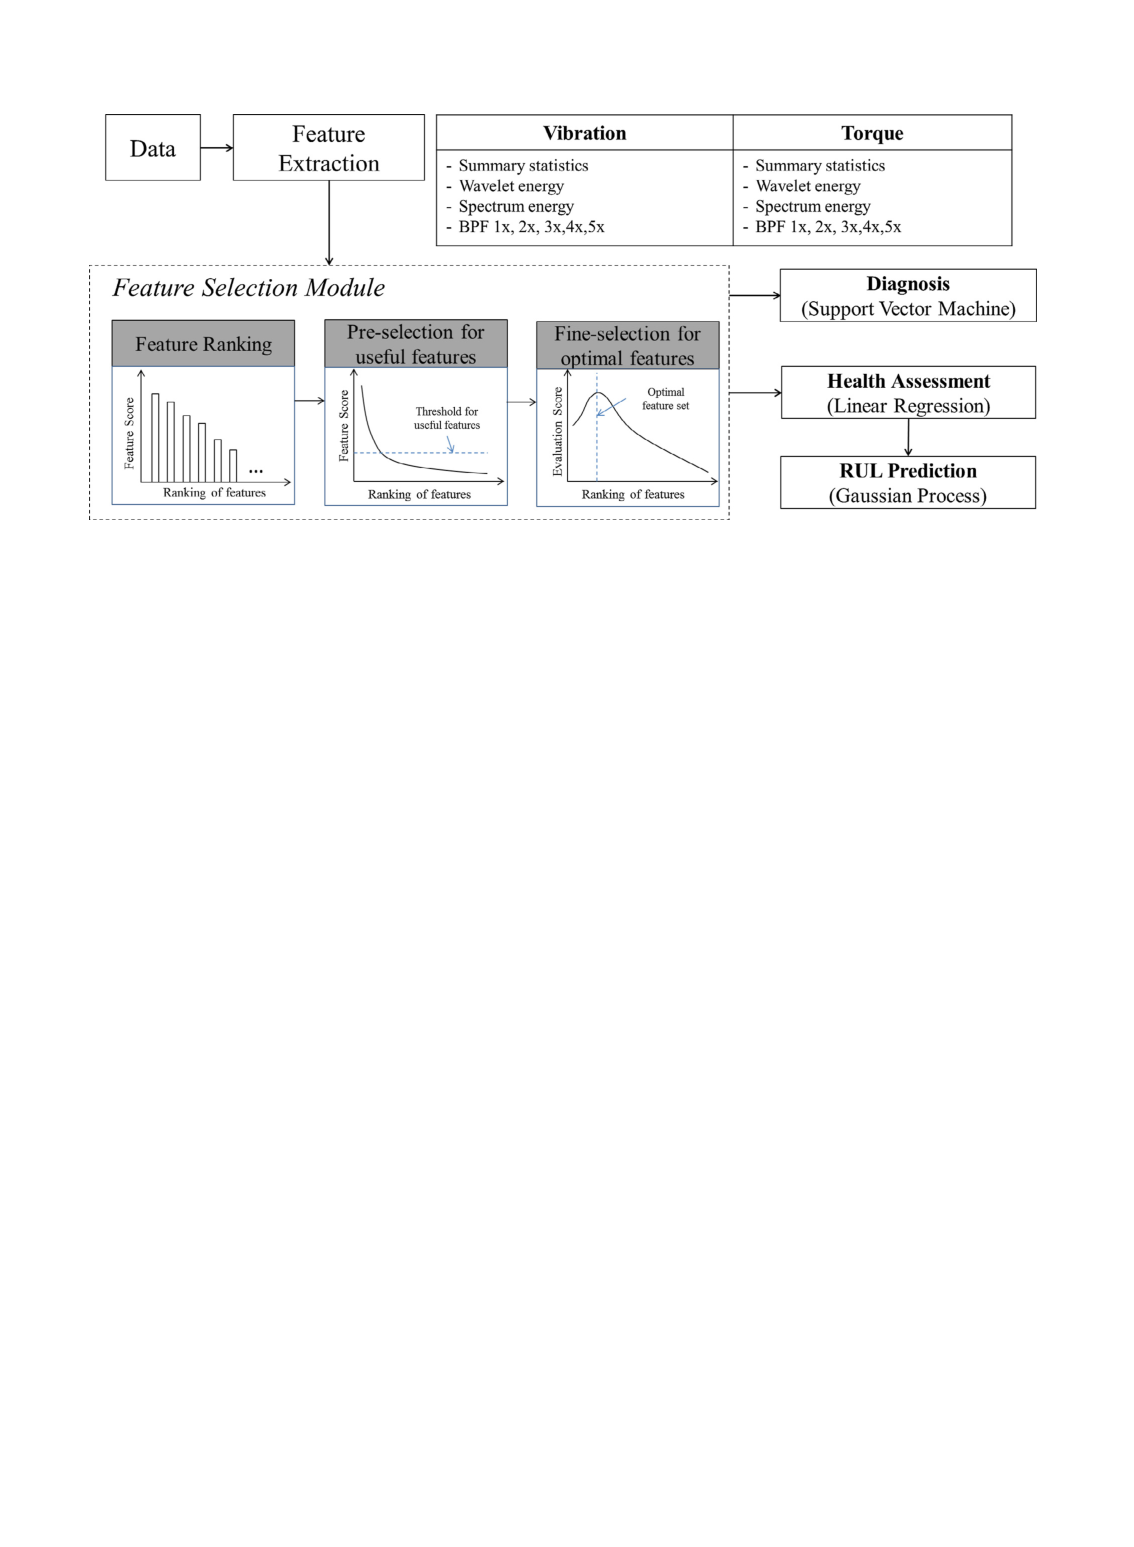
\includegraphics[width=1\textwidth]{models_state_of_the_art/model_multi-level_feature_selection.pdf}
  \caption{System architecture for multi-level feature selection module for health diagnosis, assessment and RUL prediction proposed by Li et al. \cite{LiPin2018}}
  \label{fig:level_feature_selection_model}
\end{figure}

In the following the three diagnosis steps of the proposed PHM system are presented in more detail:

\begin{itemize}
    \item [\textbf{Feature Extraction}]: The system processes the signals in the time domain, frequency domain and time-frequency domain. The wavelet decomposition (‘db4’ wavelet) is applied to transform the signals. Similarly to Denkena et al. \cite{Denkena2021}, summary statistics, such as RMS, mean, variance, kurtosis and skewness, are extracted from the signals in all three domains (time domain, frequency domain and time-frequency domain). Like in the work of Lee et al. \cite{Lee2015}, the amplitudes corresponding to the calculated ball passing frequency, as well as ball screw rotation frequency and its harmonics are extracted as features for the monitoring system \cite{LiPin2018}.
    \item [\textbf{Feature Selection}]: In a multi-level feature selection procedure the extracted features are rated by their suitability for the prognosis task. This process is separated in three stages: primary feature ranking, pre-selection and fine-selection. In order to select expressive features, a hybrid strategy of filter- (feature ranking and pre-selection) and the wrapper-based (fine-selection) approaches is applied. Wrapper methods rate features based on the performance of a classifier and filter-based methods pick features based on their intrinsic properties. In a multi-layer feature selection procedure, the search space and search sequence correspond to the features and their corresponding ranking scores found in the previous feature refinement phase. In the primary feature ranking phase, a selection criterion ranks and filters all extracted features. In the pre-selection phase, the fisher score is applied to refine the previous feature choice:
    \begin{equation}
        S_{c} = \frac{\sum_{k=1}^{C} n_{k}(\mu_{k}^{j}-\mu^{j})^{2}}{\sum_{k=1}^{C}n_{k}(\sigma_{k}^{j})^{2}}
    \end{equation}
    For the multi-class classification task the fisher score is biased. Therefore a fine feature-selection phase is added subsequently. Based on the prediction accuracy of a SVM, the final optimal features are selected \cite{LiPin2018}.
    \item [\textbf{Classification}]: A second SVM is applied to make the predictions for the diagnosis task. The SVM processes the optimal features found during the fine-selection phase \cite{LiPin2018}. 
\end{itemize}

\subsubsection{Conclusion}
From the raw data, Li et al. \cite{LiPin2018} extracted 440 features. In addition three levels of feature selection and corresponding empirical thresholds were defined. The performance of the selected features depended strongly on the signals and classification task. For the vibration signals, the expressiveness of the different features varied a lot. The performance of some features diverged strongly when being applied on the vibration and torque signals. Similarly to the work of Denkena et al. \cite{Denkena2021}, some features did not correlate well with the degradation process. The definition of the empirical threshold and application order of the different feature selection mechanism was also quite challenging. In the multi-level feature selection, the SVM-based fine-selection and fisher score-based pre-selection diverged in their feature ranking. Especially the top features found during the pre-selection were strongly down rated in the fine-selection. Defining the application order and therefore the significance of the different feature selection mechanisms, strongly influenced the final feature choice. For the 9 class classification task, finding an empirical threshold for the fisher criterion was more challenging than for the binary classification task. All these design choices are very specific and depend highly on the working conditions, class definitions and signals. Minor variations will most certainly reduce the system performance or make it even fail. Finding suitable features and selection mechanism expects a huge development effort. Using SVMs in the feature selection increases the training effort. This raises the required time and data for the model optimization. Similarly to Nguyen et al. \cite{NGUYEN2019} the physical degradation of surfaces in the BSD system was ignored. 


\section{Domain Adaptation Approaches for Prognostic and Health Management}
In recent years, more and more intelligent and adaptive data-driven approaches were proposed for monitoring the health status of industrial machines. Especially in the computer vision community, domain adaptation and transfer learning became a hot topic. Slowly models, developed in the computer vision context, also make its way in the PHM field.

\subsection{Domain Adaptation Approaches for Prognostic and Health Management of Ball Screw Drives}
In the following, deep learning-based domain adaptation approaches are presented for predicting the degradation status of BSDs. Similarly to the method proposed in this thesis, the presented models apply the MMD metric to reduce the domain discrepancy.


\subsubsection{Deep Domain Adaptation based on MMD-Loss}
Azamfar et al. \cite{AZAMFAR2020103932} proposed a deep learning-based domain adaptation approach for estimating the BSD health condition based on the preload level. The preload of the BSDs and guideways were considered as a good indication for the health condition of the components. The domain discrepancy between the training and testing dataset is reduced with a MMD-loss. An experimental test rig was build, containing a single horizontal guideway and a BSD fixed on a concrete base. Three accelerometers were installed to measure vibrations in X and Y directions. These sensors were mounted on the BSD nut and the bottom and top attachments of the BSD shaft. A sound pressure sensor captured the acoustic level when running experiments on the test rig. The torque and speed signals were acquired from the controller. Three different preload classes were defined for the guideways and BSDs. In the "normal" class the concerned component is operating normally, in the "faulty level 1" class it is deviating from the healthy condition and in the "faulty level 2" class it needs to be replaced or repaired. In total, nine combinations of guideway and BSD degradation classes were included in the PHM task. Data was recorded by performing a full cycle of BSD operation, which contains two full forward and backward movements along the guideways. The signals were split in phases with constant and changing BSD nut velocity. The training was restricted to those segments with constant BSD velocity, which were fed to the model as single samples. The data dimension was reduced by a simple down-sampling method. The recordings contained BSD operations with different BSD velocities (200, 400 and 600 mm/s). Recording the data with different BSD velocities, created a domain shift between the training and testing dataset. The proposed method was evaluated on the 9 class classification task, including all combinations of BSD and guideway degradation classes. The proposed neural network architecture is presented in fig. \ref{fig:Azamfar_model}. It contains a feature extractor of four alternating 1D convolutional and max-pooling layers and a subsequent classifier. To prevent overfitting, dropout layers with the rate of 0.3 are included. ReLU activation functions are used throughout the network. The proposed model optimization includes a source CE-loss to improve the classification accuracy on the source domain data. Besides that, the domain discrepancy is reduced by a MMD-loss, which is applied in the penultimate fully connected layer. 

\begin{figure}[H]
  \centering
  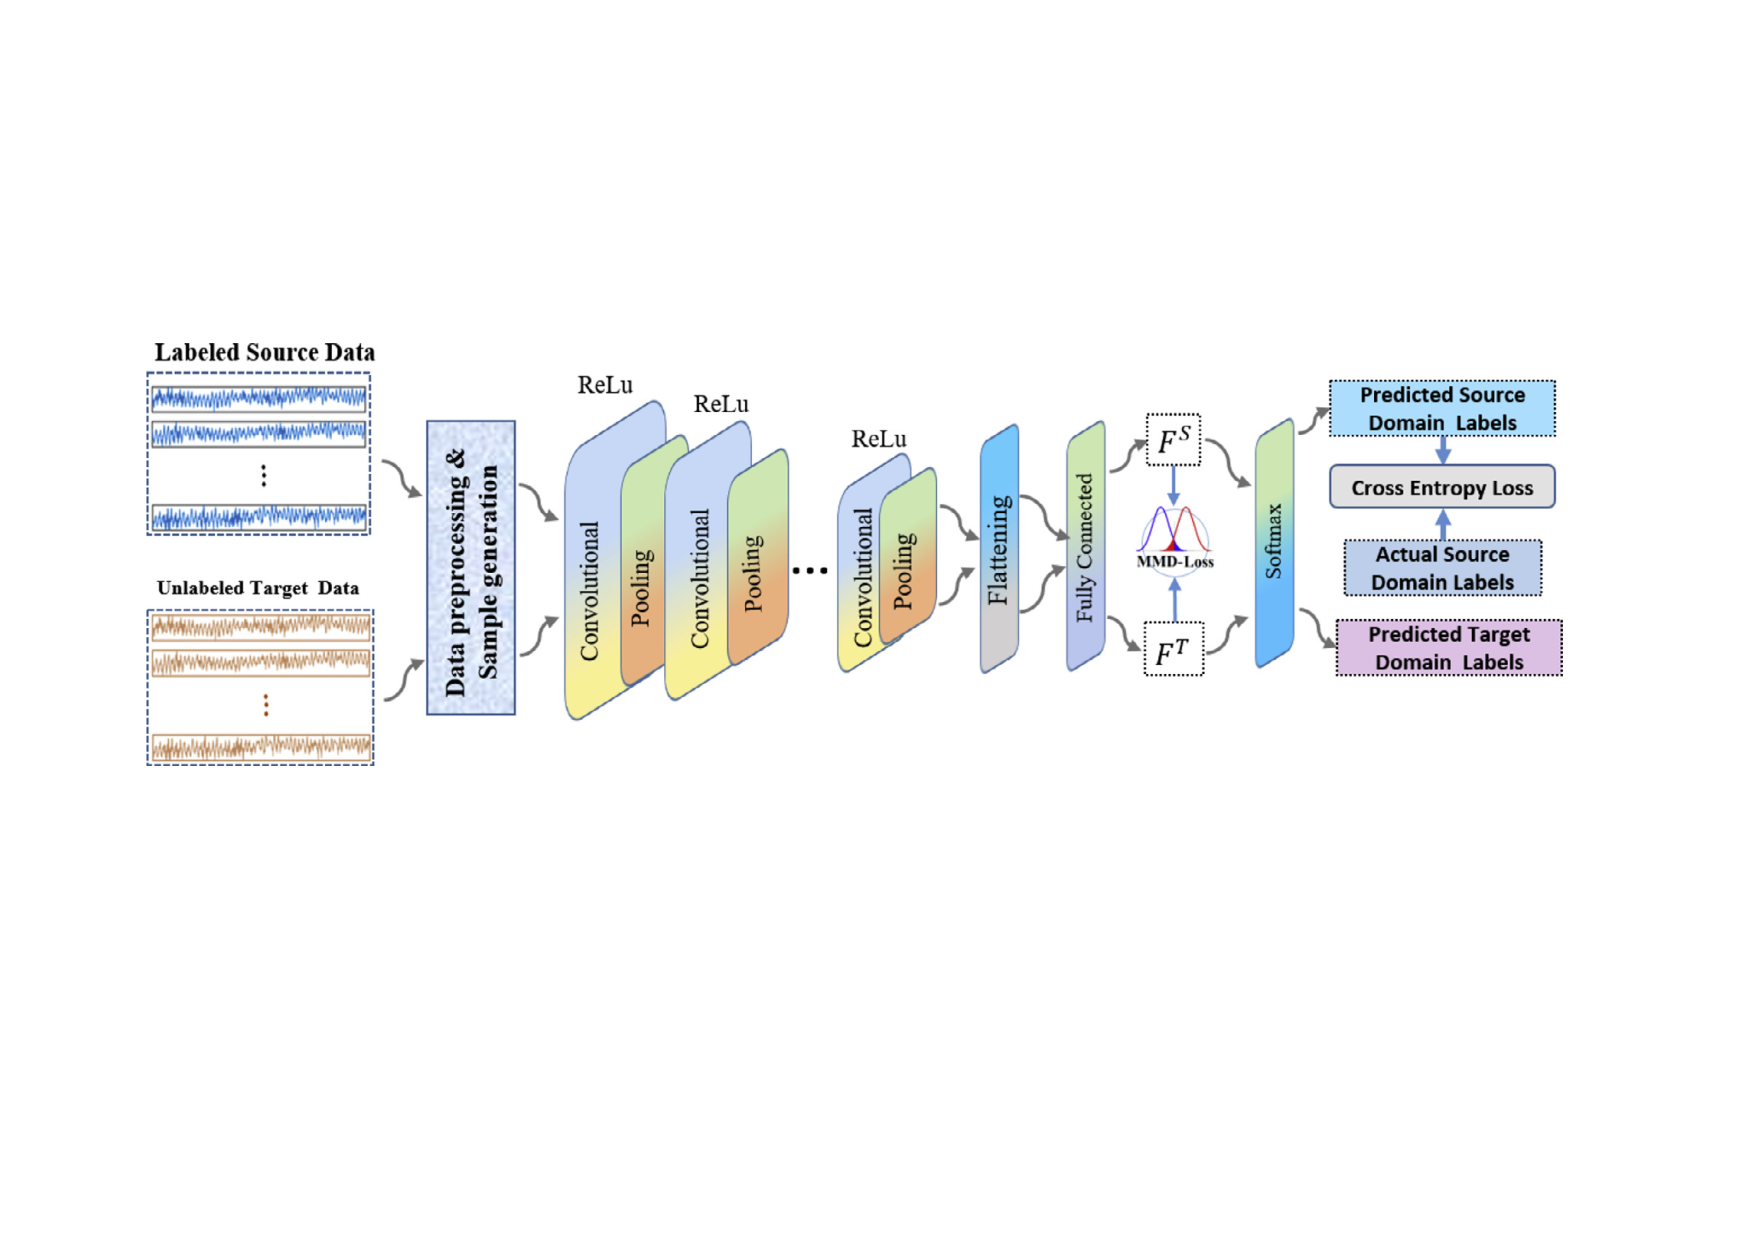
\includegraphics[width=1\textwidth]{models_state_of_the_art/Azamfar_model.pdf}
  \caption{Architecture proposed by Azamfar et al. \cite{AZAMFAR2020103932}}
  \label{fig:Azamfar_model}
\end{figure}


\subsubsection{Deep Domain Adaptation based on MMD-Loss and PD Alignment}
Similarly to Azamfar et al. \cite{AZAMFAR2020103932}, Pandhare et al. \cite{Pandhare2021} proposed a deep learning-based domain adaptation approach for estimating the BSD health condition based on the preload level. The domain discrepancy between the training and testing dataset was reduced by a MMD-loss and PD-alignment. A similar test rig, as the one presented by Azamfar et al. \cite{AZAMFAR2020103932}, was used to evaluate the proposed models. In total, five accelerometers were mounted in the testbed. Two triaxial ones were placed close to the BSD nut, which seems a promising position to represent the signature of a ball screw preload level. Three single-axial ones were mounted at the bottom and top attachments of the BSD shaft and on top of the load, carried by the BSD nut. The last three sensor positions are more suitable and practical installations. Identical to Azamfar et al. \cite{AZAMFAR2020103932}, 9 combinations of BSD and guideways preload classes were defined. By recording datasets with sensors mounted at different positions in the BSD testbed, a domain shift is created. Pandhare et al. \cite{Pandhare2021} tried to find an indirect sensing method to make PHM independent of impractical sensor locations. The proposed model architecture is presented in fig. \ref{fig:Pandhare_model} and contains a feature extractor of two alternating 1D convolutional and max pooling layers and a consecutive classifier. The proposed model training includes three losses. Again, a source CE-loss is used to improve the classification performance on the source domain data. The MMD loss reduces the marginal and the PD alignment the conditional distribution discrepancy between the domains. The PD-alignment matches source and target samples of the same class and reduces their L2-distance: 

\begin{equation}
    L_{p} = \frac{1}{n_{p}}\sum_{k=1}^{n_{p}}|h_{k}^{p,s}-h_{k}^{p,t}|_{2}, 
\end{equation}
where $h_{k}^{p,s}$ and $h_{k}^{p,t}$ are the k-th source and target domain samples and $n_{p}$ is subspace of the labeled samples from source and target. The PD-alignment is restricted to some of the 9 classes and 20\% of the training samples are used as PD samples.
\begin{figure}[H]
  \centering
  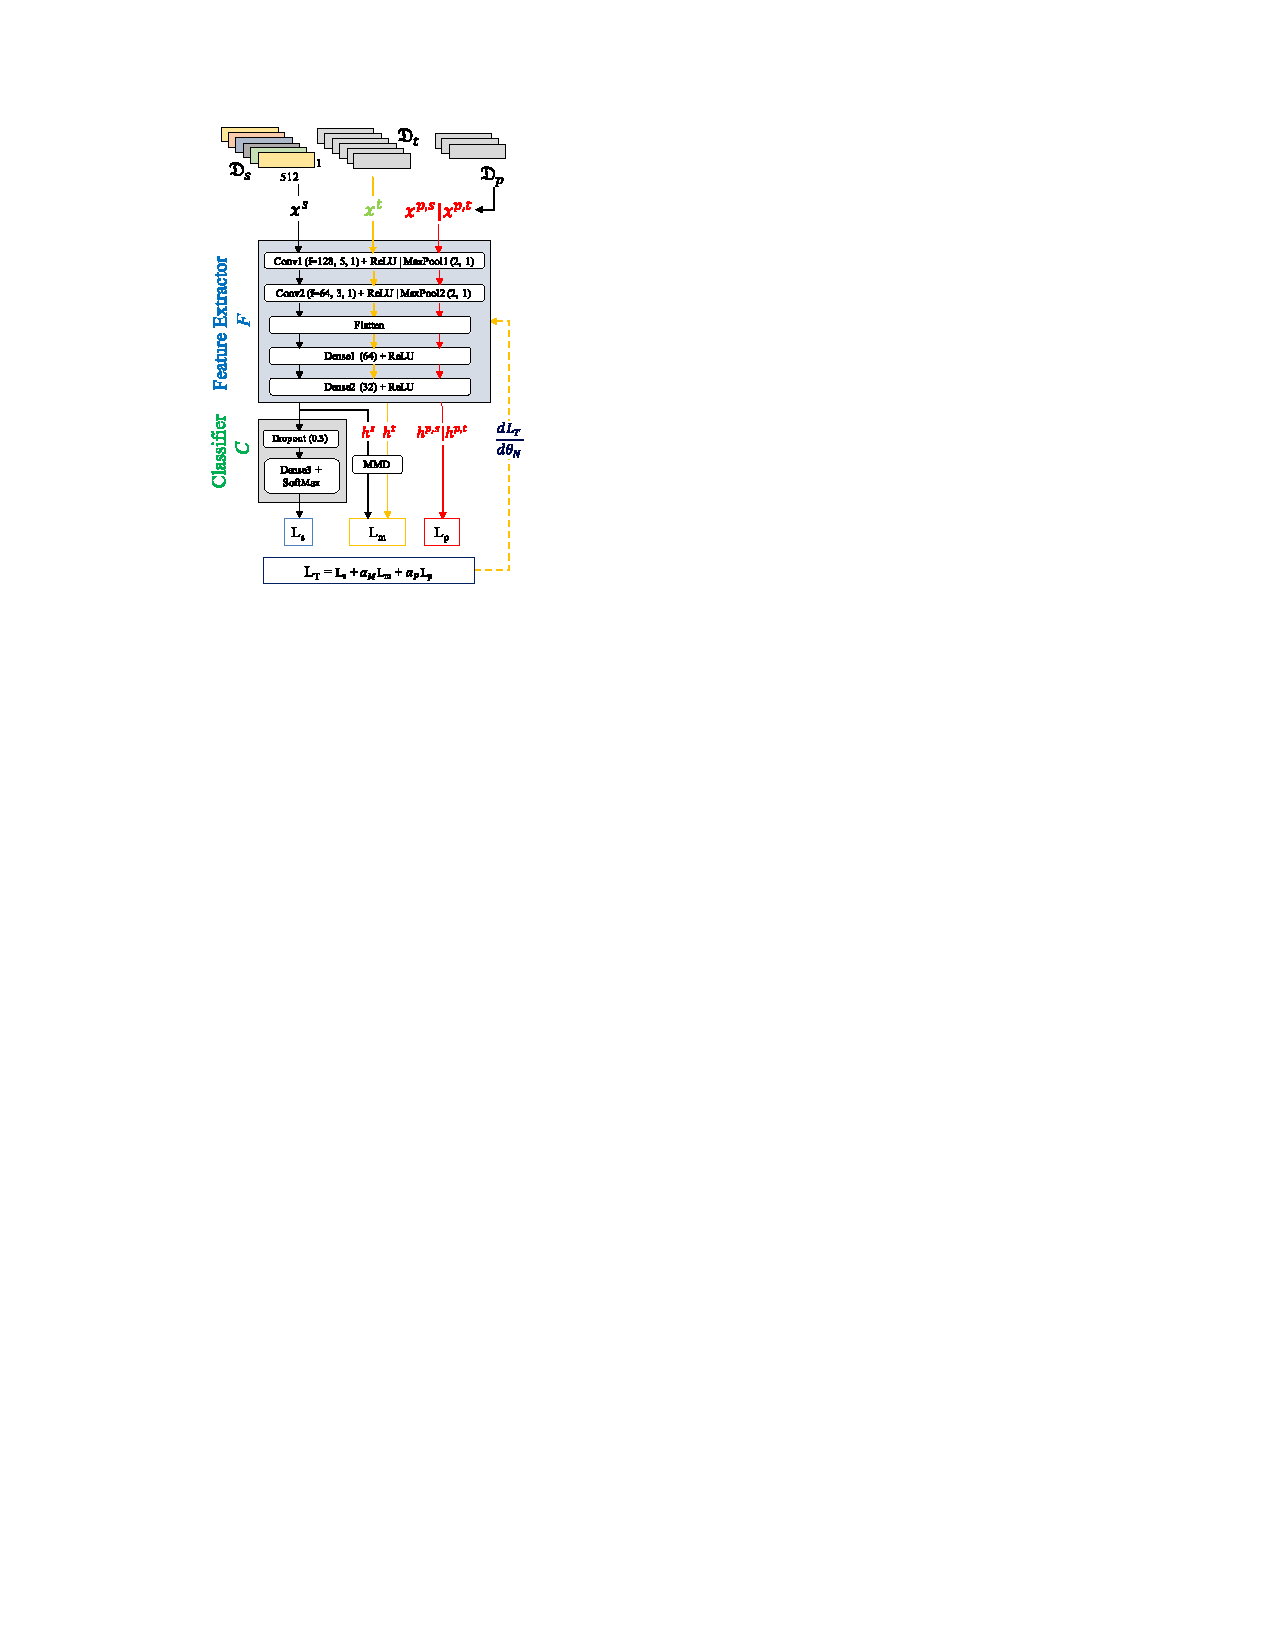
\includegraphics[width=.6\textwidth]{models_state_of_the_art/Pandhare_model.pdf}
  \caption{Architecture proposed by Pandhare et al. \cite{Pandhare2021}}
  \label{fig:Pandhare_model}
\end{figure}

\subsubsection{Conclusion}
The similar problems and disadvantages of the presented approaches by Azamfar et al. \cite{AZAMFAR2020103932} and Pandhare et al. \cite{Pandhare2021} are collectively presented in this section. First of all, both approaches apply a regime separation to separate the signals in phases of constant and changing BSD velocity. This extra step adds additional complexity to the data pre-processing. Both approaches avoid windowing the signals. The segments with constant BSD velocity are fed to the models as single samples. Since those samples capture the frequency and amplitude variations during the whole steady-state phase of the BSD operation, they are assumed to be more informative for the monitoring task. By doing so just a few samples are collected from each recorded experiment. A lot of experimental effort is required to record enough samples to properly train the neural network. Azamfar et al. \cite{AZAMFAR2020103932} and  Pandhare et al. \cite{Pandhare2021} evaluate their monitoring approaches solely on a simplified testbed. Therefore, the evaluation of the approaches did not consider the mutual influence of other components installed in real industrial machines. Besides that, both approaches are restricted to predict BSD preload forces. Other damages like pitting were ignored by the monitoring systems. In both cases the MMD-loss was just applied in the last fully connected layer without evaluating other latent feature spaces for their suitability to reduce the domain discrepancy. Azamfar et al. \cite{AZAMFAR2020103932} created a domain shift by recording data with different BSD velocities and Pandhare et al. \cite{Pandhare2021} by recording data with accelerometers mounted at different positions in the BSD testbed. In both cases the domain shift did not include any differences on the physical component level. The same components were represented in the two domains and therefore also training and testing dataset. The PHM systems did just have to deal with domain shifts created by variations in the BSD operational conditions and data recording. It was not evaluated how the presented approaches react to physical variations in the systems. The PD-alignement approach, presented by Pandhare et al.  \cite{Pandhare2021}, expects target labels from some of the considered classes, which simplifies the health monitoring task and is impratical for real-world PHM systems.

\subsection{Domain Adaptation Approaches for Prognostic and Health Management of Rolling Bearings}

A PHM algorithm for rolling bearings, which optimizes the inter- and intra-class distance in the latent feature space and reduces the domain discrepancy with a MMD-loss, was presented by Li et al. \cite{Li2018}. As visualized in fig. \ref{fig:Deep_distance_metric_learning_model}, the proposed model contains a CNN and a consecutive classifier. In a preprocessing step, a FFT transform is applied to represent the raw vibration signals in the time-frequency domain. Max-pooling layers are included to reduce the model size. Batch-normalization layers reduce the internal covariate shift by normalizing the input distributions of the hidden layers. To prevent overfitting, dropout layers with a rate of 0.5 are included. The proposed method was evaluated on a rolling bearing dataset provided by the Bearing Data Center of Case Western Reserve University. The domain shift was generated by using testing data, which was exposed to additional environmental noise and collected under different working conditions. 10 health conditions with faults in different location and with different extent were defined. 

\begin{figure}[H]
  \centering
  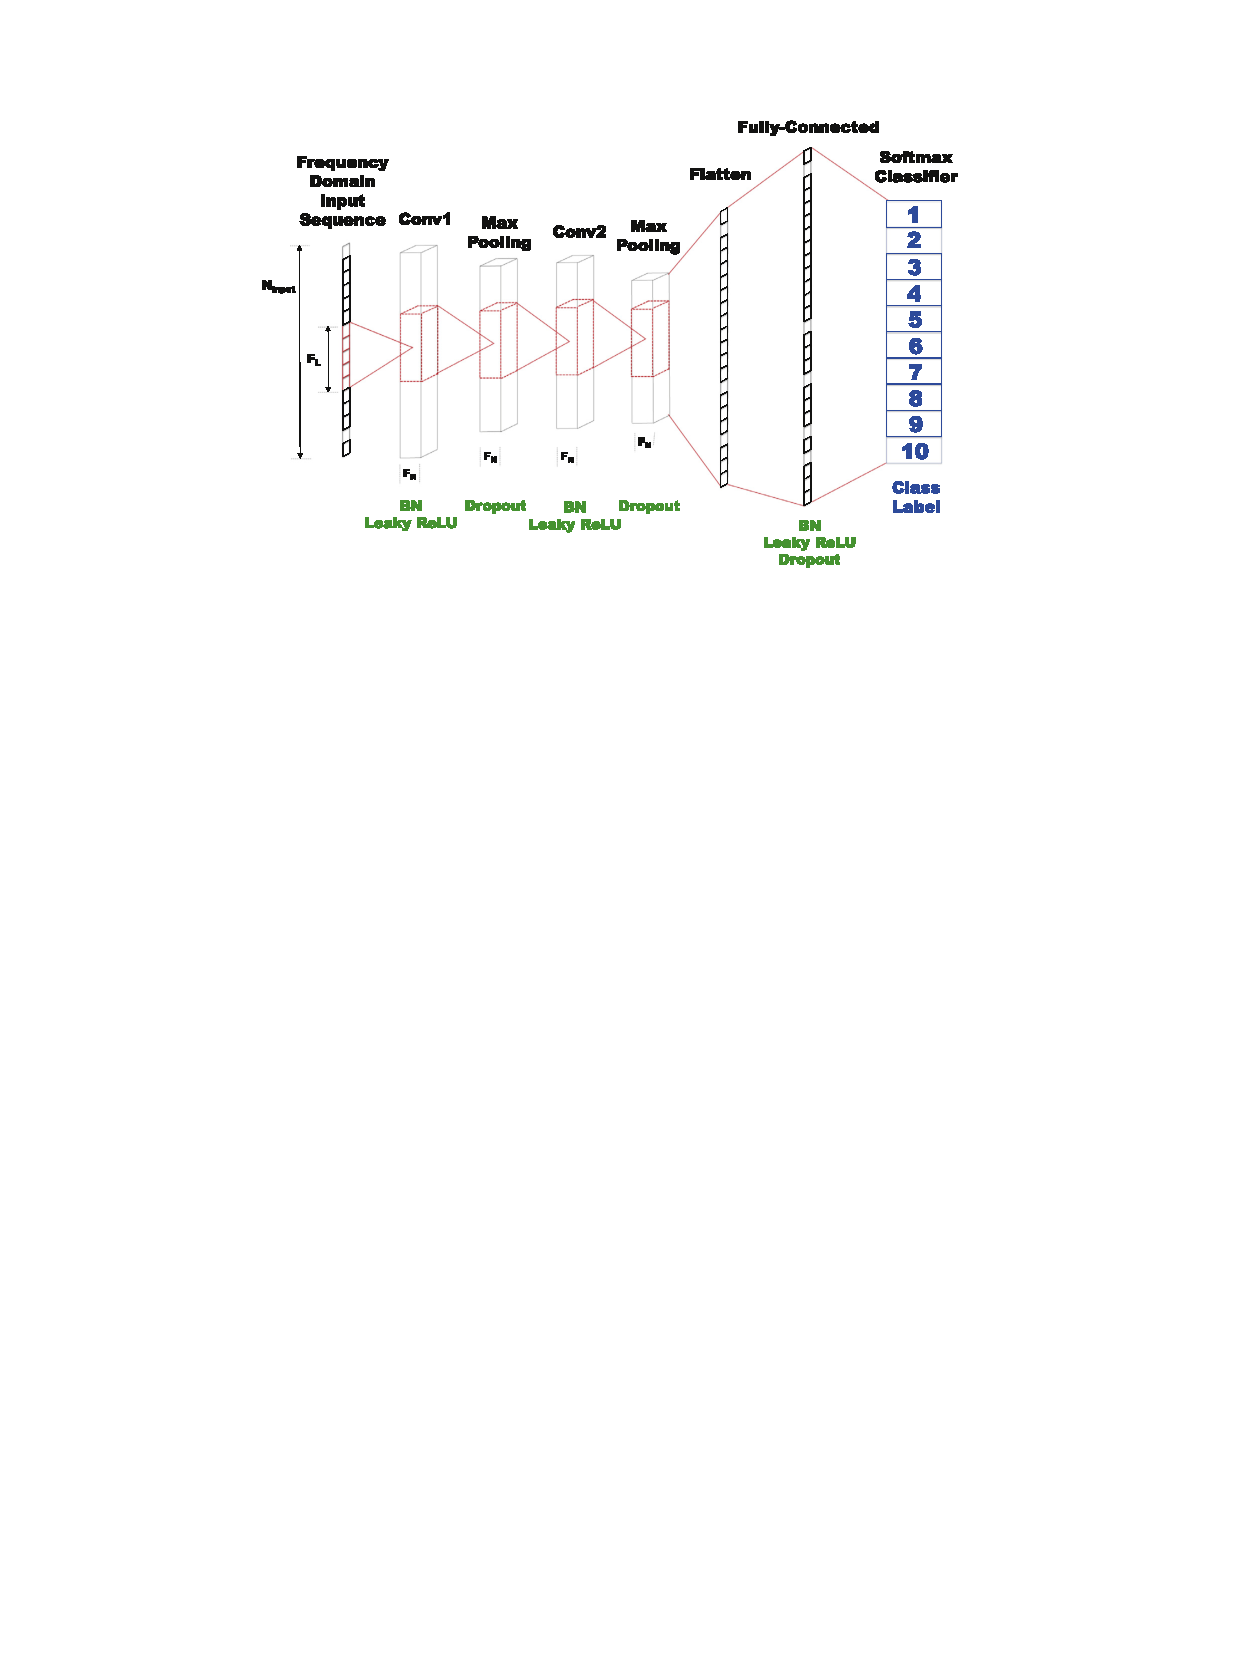
\includegraphics[width=.75\textwidth]{models_state_of_the_art/Deep_distance_metric_learning_model.pdf}
  \caption{Deep distance metric learning architecture proposed by Li et al \cite{Li2018}}
  \label{fig:Deep_distance_metric_learning_model}
\end{figure}

Li et al. \cite{Li2018} suggested to optimize the model such that the distance between the source samples is minimized if they belong to the same class and maximized otherwise. This increases the separability and compactness of the source domain classes, which makes the algorithm more robust against environmental noise. In order to calculate the intra- and inter-class distances, the expectation and variance of the source domain samples belonging to the same class is measured in the feature maps:

\begin{equation}
    \begin{aligned}
       &D_{inter} = |E[f^{(m)}x^{(i)}]-E[f^{(m)}x^{(j)}]|_{2}-\sqrt{Var[f^{(m)}x^{(i)}]}-\sqrt{Var[f^{(m)}x^{(j)}]}\\
       &D_{intra} = 
        \sum_{i=1}^{N_{class}} \sqrt{Var[x^{(i)}]},
    \end{aligned}
\end{equation}

where $N_{class}$ is the number of classes, $x^{(k)}$ denotes the raw input sample of class k, $f^{(m)}x^{(k)}$ denotes the feature representation of this sample in the m-th layer and $E[f^{(m)}x^{(i)}]$ and $Var[f^{(m)}x^{(i)}]$ are the corresponding expectation and variance. The inter- and intra-class distance are optimized with the following loss: $J_{Cluster} = - D_{inter} + \eta D_{intra}$. In addition to the distance metric learning, the discrepancy between the source and target domain is reduced by an MMD-loss in several FC layers. Lastly, the network is optimized by a CE-loss in the final layer to classify the source samples correctly. In total, the network is optimized with the following weighted average of losses: 

\begin{equation}
    \begin{aligned}
    J_{total} = \alpha J_{Cluster} + \beta J_{MMD} + \gamma J_{CE}, 
    \end{aligned}
\end{equation}
where $J_{Cluster}$ is the loss optimizing the distances between the source domain samples, $J_{MMD}$ the MMD-loss,  $J_{CE}$ the CE-loss and $\alpha$, $\beta$ and $\gamma$ are the weights for calculating the weighted average \cite{Li2018}.

\subsubsection{Conclusion}
There are several domain adaptation approaches for PHM of rolling bearing based on MMD-losses \cite{AN201942} \cite{Li2018} \cite{Guo2019} \cite{Singh2019} \cite{Kang2020}. Generally, BSDs and rolling bearing are related components. BSD shafts can be seen as the inner and BSD nuts as the outer ring of rolling bearings. In both cases balls between those two components allow a rotatory motion around a fix axis. Other than rolling bearings, BSDs also translate this rotatory motion in a linear motion. The degradation of rolling bearings and BSDs is related in some sense. Nevertheless, bearing PHM applications cannot be relied to work as well for BSDs. Still the research in this domain offers interesting applications and details for the PHM of BSDs. 

\section{Feature Extractor Based Domain Adaption in Computer Vision Applications}

\begin{comment}
\subsection{Domain Conditioned Adaptation Network}
Li et al. \cite{li2020} propose a domain conditioned adaptation network (DCAN), which contains two separate modules to reduce the domain discrepancy. After each task-specific layer a domain conditioned feature correction block estimates and reduces the domain discrepancy based on the MMD metric. In the CNN backbone an attention module regulates the extraction of domain-specific and -independent features. The proportions of domain-specific and -independent features is learned to decrease the domain discrepancy. Fig. \ref{fig:DCAN_model} visualizes the domain adaptation modules in the DCAN model.

\subsubsection{Domain Conditioned Channel Attention Mechanism}
ResNet is used as a backbone network, which allows an easy implementation of the domain conditioned channel attention module in its residual block. In the latent feature maps, the processed images are represented as $\pmb{X}_{t} = [X^{1}_{t},...,X^{C}_{t}] \in \mathbb{R}^{HxWxC}$, where H and W are the spatial dimension and C the number of image channels. First, a channel-wise global average pooling layer is applied, which reduces the images to  $\pmb{g}_{t} = [g^{1}_{t},...,g^{C}_{t}] \in \mathbb{R}^{1x1xC}$. Afterwards, the data is split depending on its domain and passed through different fully connected layers. The upper flow is used for target and the lower flow for source domain samples. The two different source and target domain routes share parameters. For both domains, an attention mechanism is trained jointly to learn activating different channels in the domain samples. This allows extracting more enriched domain-specific features. In the fully connected layers the dimension is first reduced with a ratio ${1x1x\frac{C}{r}}$ and later reconstructed to its original size ${1x1xC}$. ReLU and Sigmoid functions are applied. The domain-wise feature selection is achieved by weighting the channels of the feature representations $\pmb{X}_{s}$ and $\pmb{X}_{t}$ with the channel attention vectors $\pmb{v}_{s}$ and $\pmb{v}_{t}$ calculated by the domain conditioned channel attention module:

\begin{equation}
    \begin{aligned}
        &\pmb{\tilde{X}}_{s} = \pmb{v}_{s} \odot \pmb{X}_{s} = [v_{s}^{1} \cdot X_{s}^{1}, ..., v_{s}^{C} \cdot X_{s}^{C}]\\
        &\pmb{\tilde{X}}_{t} = \pmb{v}_{t} \odot \pmb{X}_{t} = [v_{t}^{1} \cdot X_{t}^{1}, ..., v_{t}^{C} \cdot X_{t}^{C}].
    \end{aligned}
\end{equation}

The domain conditioned channel attention module allows the model to independently learn the importance of each channel for the classification of source and target domain samples \cite{li2020}.

\subsubsection{Domain Conditioned Feature Correction}
The data simultaneously passes through the regular network and the feature correction block, which consist of FC and ReLU blocks. The feature correction block estimates the domain discrepancy in the feature representation of the task-specific layer:
\begin{equation}
    \Delta H_{l}(x_{t}) = H_{l}(x_{s}) - H_{l}(x_{t}),
\end{equation}
where $H_{l}(x_{s})$ and $H_{l}(x_{t})$ are the feature representations of the source and target domain samples in the task-specific layer l. $\pmb{x}_{s}$ and $\pmb{x}_{t}$ are the source and target domain samples. The feature representation of the target domain samples is corrected as following:

\begin{equation}
    \hat{H}_{l}(x_{t}) = H_{l}(x_{t}) + \Delta H_{l}(x_{t}).
\end{equation}

The discrepancy between the regular feature representation of source domain samples $H_{l}(x_{s})$ and the corrected feature representation of the target domain samples $\hat{H}_{l}(x_{t})$ is measured by the MMD-loss in several layers:

\begin{equation}
    L_{M}^{l} = |\frac{1}{n_s} \sum_{i=1}^{n_{s}} \phi(H_{l}(x_{si}) - \frac{1}{n_t} \sum_{i=1}^{n_{t}} \phi(\hat{H}_{l}(x_{ti}))|_{H_{\kappa}}^{2}, 
\end{equation}
where $H_{\kappa}$ is the reproducing kernel Hilbert space (RKHS), $\kappa$ the characteristic kernel and $\phi$ the corresponding feature map. The number of source and target samples is defined by $n_{s}$ and $n_{t}$. To avoid the over-transfer of noise and irrelevant information between source and target, the model is enforced to keep the source data constant when passing through the feature correction blocks \cite{li2020}.

\begin{figure}[H]
  \centering
  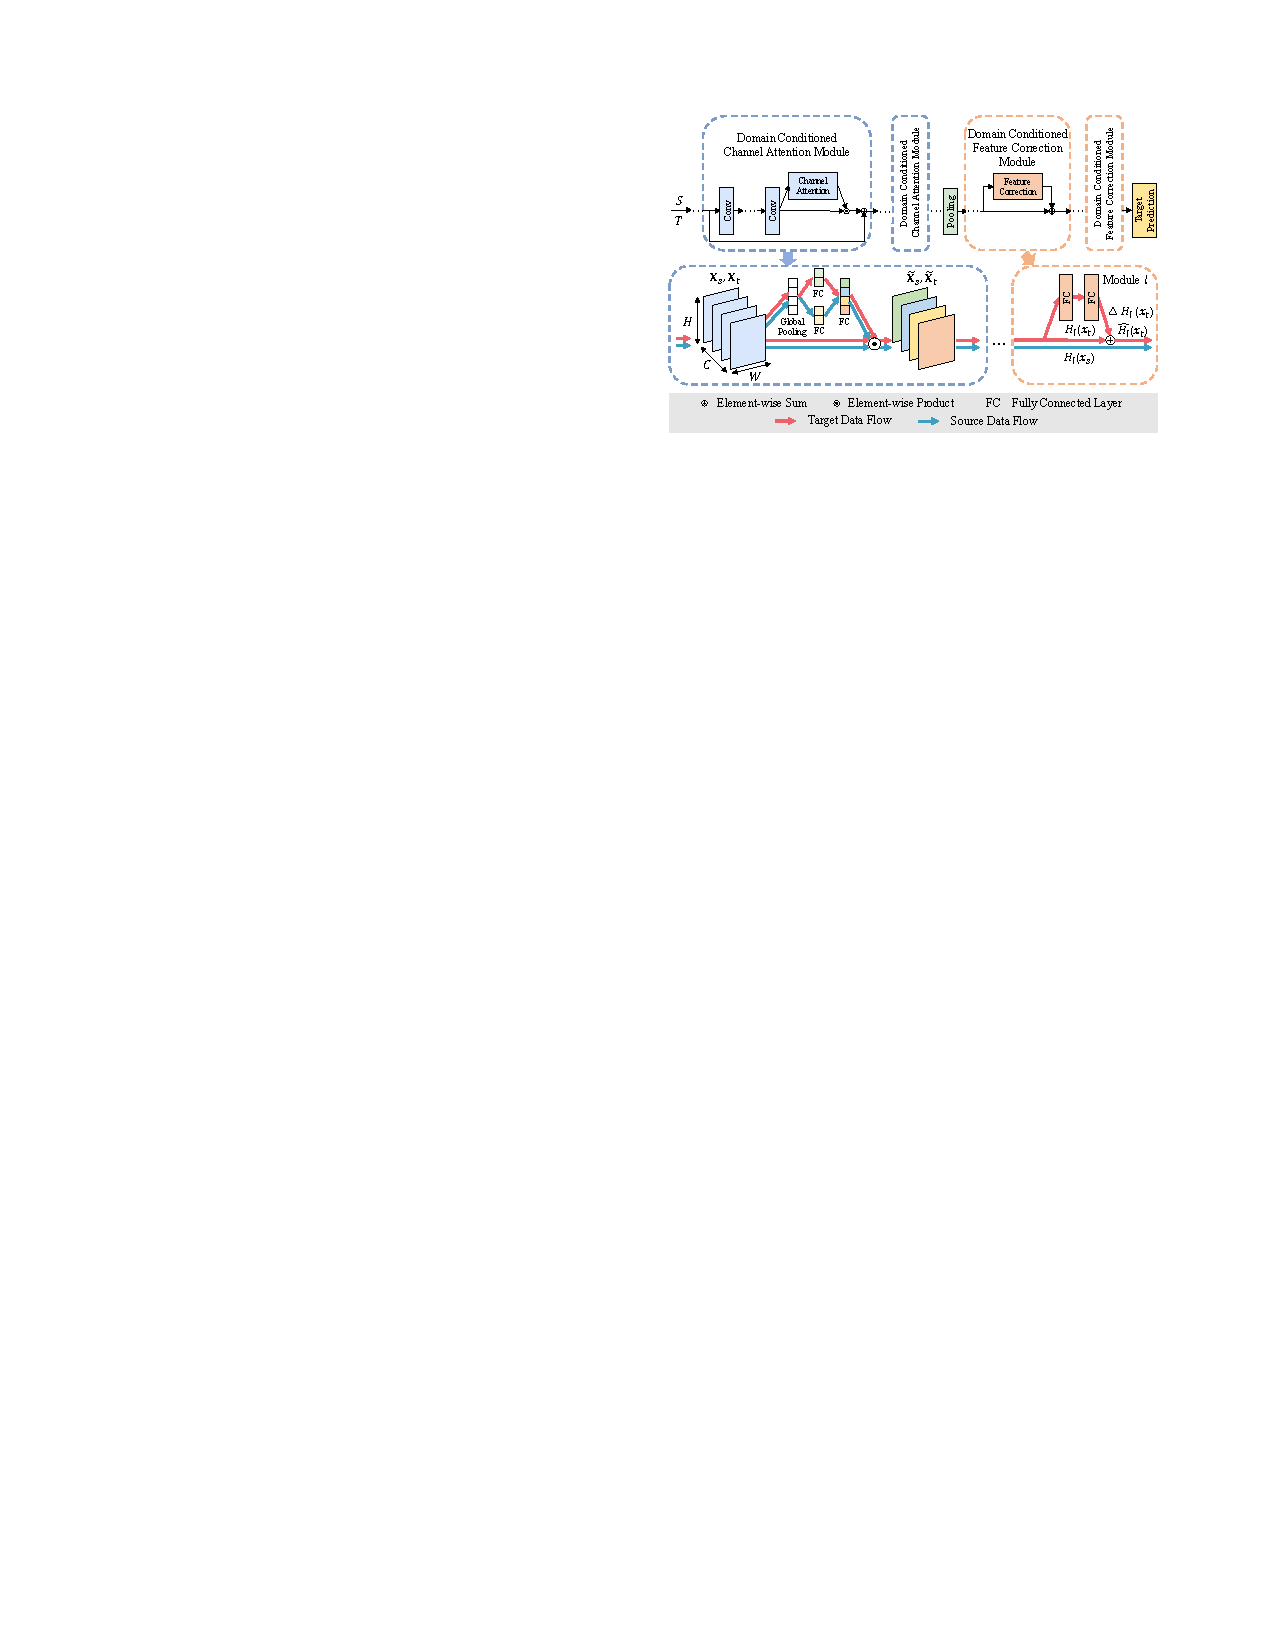
\includegraphics[width=1\textwidth]{models_state_of_the_art/DCAN_model.pdf}
  \caption{DCAN architecture proposed by Li et al. \cite{li2020}}
  \label{fig:DCAN_model}
\end{figure}

\end{comment}

%\subsection{Feature Reconstruction of Domain Shift Affected Layers}
Aljundi et al. \cite{Aljundi2016} presented a domain adaption approach for computer vision application. The method analyzes the output of all convolutional layer for domain shift effects. The goal is to find the layers which suffer most from those effects. By reconstructing affected latent feature space outputs, the new target sample outputs should become more similar to the response given for the source samples. In a first step, the domain shift effects with respect to each layer are measured:
\begin{equation}
    B^{*} = argmin_{B} \{ \sum_{i=1}^{n}( y_{i}-\beta_{0}-\sum_{j=1}^{p}x_{i,j}\beta_{j})^{2} + \lambda \sum_{j=1}^{p}|\Delta_{j}^{KL}\cdot \beta_{j}| \}
\end{equation}
where y is the response, x the output of the various layers, $\beta_{0}$ the residual, $B = \{\beta_{j}\}$ the estimated coefficients for each layer, n the number of
source samples, p the number of layers, $\lambda$ a tuning parameter to punish the value of the coefficients and $\Delta_{j}^{KL}$ the KL divergence measured between the source and target data representation in each layer. When a layer's coefficient  $\beta_{j}$ is big, it is considered as good (small domain shift effects) and otherwise as bad (big domain shift effects). The optimization is solved by using the coordinate descent method. In a second step, linear regression is applied to predict new coefficients for the good layers to replace the output of the bad ones. The reconstructed layer outputs are then passed to the subsequent layers. Aljundi et al. \cite{Aljundi2016} identified that especially the early layers of the feature extractor are relevant to counteract the domain shift.

\subsubsection{Conclusion}
The presented approach by Aljundi et al. \cite{Aljundi2016} disagrees with most domain adaptation approaches, which reduce the domain discrepancy in task-specific layers but use a shared feature extractor backbone across all domains. The work shows the positive effect of reducing the domain shift in early layers of the feature extractor. Often times there is no clear pattern of which layers contribute most to the domain discrepancy problem. It is therefore a great approach to evaluate each layer individually and to adapt the domain reduction adequately. The work shows, that early layers in the feature extractor already suffer from and significantly contribute to the domain shift. Often the computer vision community offers advanced solution for complex research questions, which were not intensively evaluated in real-world scenarios. For the PHM of BSDs such solutions can be taken as inspiration. 

\section{Research Gap}
When industrial machines run over long time horizons, fault characteristics might change due to variations in the operational conditions, changed machine settings, minor installation differences after replacing submodules or physical degradation. Due to the mutual influence of different machine submodules, fault characteristics are often complex and highly dependent. Developing hand-crafted features, as they are quite common in traditional approaches, expect a lot of experience and human labor. Due to the lack of flexibility and robustness, hand-crafted features struggle to extract expressive information from the data when the corresponding fault characteristics change over time. Li et al. \cite{Lee2015} estimate the degradation and Nguyen et al. \cite{NGUYEN2019} the preload of BSDs, based on simplified models. The quality of model-based PHM systems highly depends on the exactness and sophistication of the underlying modeling and the corresponding parameters. If the model misses details from the real-world machines and processes, the PHM performance will decrease over time. Data-driven PHM systems, like those proposed by Denkena et al. \cite{Denkena2021} and Li et al. \cite{LiPin2018}, might find more general and expressive features, which are less prone to small variations in the fault characteristics. Adapting such systems to new circumstances is often less time-consuming since these models learn the correlation between the machine data and health condition classes automatically. Anyhow, the performance of such systems highly depends on the underlying training dataset. It is unlikely that the data used for training includes all operational conditions and fault scenarios. It can even happen that fault classes are unknown during training. Training neural networks on a limited amount of data, which does not represent the data distributions during testing, might lead to an unsatisfactory diagnosis performance \cite{AZAMFAR2020103932}. Robust PHM systems, which can handle variations in fault characteristics, would bring industrial PHM systems to a next level \cite{Michau2017}. In order to address those issues, domain adaptation seems promising for PHM systems. This thesis investigates the applicability and usability of deep learning-based domain adaptation for the health monitoring of BSDs. The advantages of the proposed systems over regular deep learning-based systems are evaluated. Since it expects a lot of work to establish accurate model-based PHM approaches, the developed approaches in this thesis could not be compared with such systems. 